\chapter{NB-IOT通信技术基础}
时域积分方程(TDIE)方法作为分析瞬态电磁波动现象最主要的数值算法之一,常用于求解均匀散射体和表面散射体的瞬态电磁散射问题。

\section{AT指令}
AT指令集用于从终端设备或数据终端设备通过终端适配器向控制移动台发送控制指令,3GPP TS 27.007 规定了用于控制GSM手机或者modem的AT命令,比如 AT+CIMI 用于获取设备的IMEI(Intemational Mobile Subscriber Identity),AT+CSQ 用于获取信号强度;3GPP TS 27.005 规定了管理GSM和SMS短信功能的指令,例如AT+CNGC用于发送SMS短信;模块通用指令比如 AT+NRB用于重启模块;还有用于特定IOT平台的命令,比如AT+NCDP用于查询华为IOT平台CDP服务器的IP/端口。
AT指令为以下四种形式

\begin{table}[h!]
\caption{AT指令形式}
\begin{tabular}{lll}
\toprule
类型&形式&解释\\
\midrule
测试指令&AT+<cmd>=?&获取参数可能的值范围\\
读取指令&AT+<cmd>?&读取参数值\\
写指令&AT+<cmd>=p1,[p2,[p3[......]]]&设置参数值\\
执行指令&AT+<cmd>&执行命令\\
\bottomrule
\end{tabular}
\label{AT指令形式}
\end{table}


\section{NB-IOT模块的工作状态}
NB-IOT省电的特点,很大程度得益于3种工作模式的切换,通过牺牲一定的实时性,停止一部分功能,从而达到省电目的。NB-IOT三种工作模式的切换如下图所示(补充图片)
当NB-IOT模块注册入网后,处于connected态,此时模块可以收发数据,当无上行数据后,启动不活动定时器,到期后进入IDLE态,开始TAU计时,关闭发射,保留接收功能,可对下行数据进行处理,如有下行激活指令,则切换到connected态,否则active timeer到期后进入PSM态,关闭收发功能,仅保留必要的时钟。TAU到期后切换到connected态

\section{工作频段}
NB-IOT沿用LTEd定义的频段号,Release 13 为NB-IOT制定了14个频段,国内运营商的NB-IOT设备主要运行在band 5 和 band 8


\begin{table}[h!]
\caption{运营商band分配}
\begin{tabular}{ccccc}
\toprule
频段&中心频率&上行频率&下行频率&\multirow{2}{*}{运营商}\\
(MHZ)&(MHZ)&(MHZ)&(MHZ)&\\
\midrule
Band 5&850&824-849&869-894&中国电信\\
\midrule
Band 8&900&880-915&925-960&\makecell[c]{中国移动\\中国联通}\\
\bottomrule
\end{tabular}
\label{运营商band分配}
\end{table}


\section{部署方式}
NB-IOT支持带外、带内和保护带部署三种方式

\section{信令协议}

\section{应用层协议}

物联网设备多为系统资源受限设备,对网络的要求也与普通互联网应用有很大不同。目前流行的为物联网受限设备设计的应用层协议主要是CoAP、MQTT-SN、XMPP、AMQP等(TODO:引用)。接下来对应用更为广泛的CoAP和MQTT协议进行对比。

\subsection{CoAP}
CoAP与http一样,基于REST架构的应用层协议,但传输层使用UDP替换,自身则是一个双层结构(消息层和请求响应层),并在消息层实现了多播、拥塞控制、消息可靠性保证等机制。作为一个轻量级协议,CoAP协议的最小报文仅为4字节.

\begin{figure}[h]
	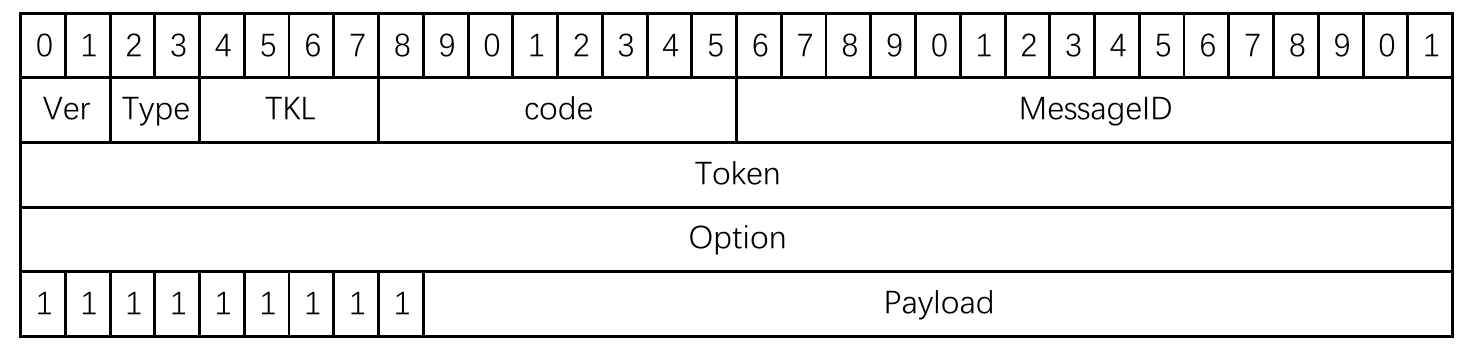
\includegraphics[width=14cm]{CoAP报文.png}
	\caption{CoAP的消息格式}
	\label{CoAP报文}
\end{figure}

  
\begin{table}[h!]
\caption{CoAP字段}
\begin{tabular}{ccc}
\toprule
字段名 & 比特数 & 解释\\
\midrule
Ver&2&代表协议版本,目前为 0x01 \\
Type&2&\makecell[c]{消息类型,CON为可靠传输,需要响应,响应消息类\\型为 ACK 和 RSTNON 为不可靠传输,不需要响应}\\
TKL&4&Token 的长度,目前为 0~8B \\ 
Code&8&	\\
MessageID&16&消息ID,用于标记重发消息\\
Token&&可选,长度为TKL,用于消息安全性或对应一个请求和响应\\
\bottomrule
\end{tabular}
\label{coap字段}
\end{table}


\subsection{MQTT}

MQTT是一种发布/订阅传输协议,基于TCP/IP协议栈构建,具有低开销,低带宽占用的优点,协议中有三种身份:publisher、broker和subcriber,broker起到解耦合的作用。MQTT提供三种消息传递的服务质量水平:

\begin{table}[h!]
\caption{MQTT服务质量}
\begin{tabular}{cc}
\toprule
值 & 解释 \\
\midrule
0 & a \\
1 & b \\
2 & c \\
\bottomrule
\end{tabular}
\label{tablea}
\end{table}



\begin{table}[h]
\caption{计算$2m\times 2m$理想导体平板时域感应电流采用的三种存储方式的存储量比较。}
\begin{tabular}{cccc}
\toprule
\multirow{2}{*}{时间步长} & \multicolumn{3}{c}{存储方式} \\
\cmidrule{2-4}
& 非压缩存储方式 & 完全压缩存储方式 & 基权函数压缩存储方式 \\
\midrule
0.4ns & 5.59 MB & 6.78 MB & 6.78 MB\\
0.5ns & 10.17 MB & 5.58 MB & 5.58 MB \\
0.6ns & 8.38MB & 4.98 MB & 4.98 MB \\
\bottomrule
\end{tabular}
\label{tablea}
\end{table}

\begin{figure}[h]
	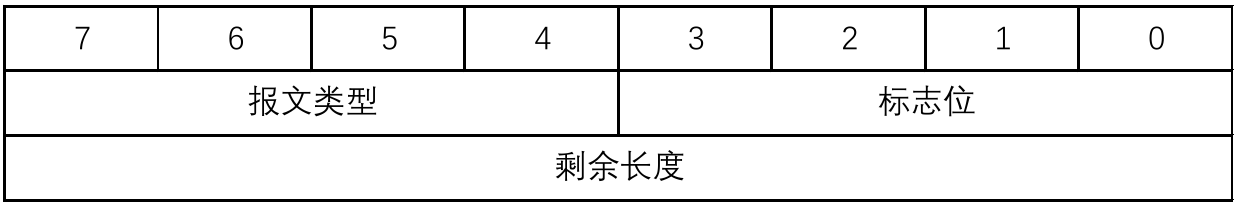
\includegraphics[width=12cm]{MQTT报文.png}
	\caption{MQTT报文结构}
	\label{MQTT报文}
\end{figure}

\begin{table}[h!]
\caption{MQTT报文字段}
\begin{tabular}{ccl}
\toprule
字段名 & 比特数 & 解释\\
\midrule
Control Packet type	&4&控制报文类型,4位无符号数\\
Flags	&4&	\\
Remaining Length&&\makecell[c]{剩余长度表示当前报文余下的负载数据长度\\(不包含自身),使用Base 128 Varints编码}\\
\bottomrule
\end{tabular}
\label{mqtt字段}
\end{table}

\subsection{CoAP和MQTT的异同}


  MQTT协议使用发布/订阅模型,CoAP协议使用请求/响应模型;

  MQTT会通过网关在客户机之间创建连接,CoAP协议则是无连接协议;

  MQTT通过中间代理传递消息的多对多协议,CoAP协议是Server和Client之间消息传递的单对单协议;
  
  MQTT不支持带有类型或者其它帮助Clients理解的标签消息,CoAP内置内容协商和发现支持,允许设备彼此窥测以找到交换数据的方式。

\begin{equation}
f_n(\bm{r})=
\begin{cases}
\frac{l_n}{2A_n^+}\bm{\rho}_n^+=\frac{l_n}{2A_n^+}(\bm{r}-\bm{r}_+)&\bm{r}\in T_n^+\\
\frac{l_n}{2A_n^-}\bm{\rho}_n^-=\frac{l_n}{2A_n^-}(\bm{r}_--\bm{r})&\bm{r}\in T_n^-\\
0&\text{otherwise}
\end{cases}
\end{equation}

其中,$l_n$为三角形单元$T_n^+$和$T_n^-$公共边的长度,$A_n^+$和$A_n^-$分别为三角形单元$T_n^+$和$T_n^-$的面积(如图\ref{pica}所示)。

\begin{figure}[h]
	\includegraphics{pica.pdf}
	\caption{AT指令形式}
	\label{p}
\end{figure}

由于时域混合场积分方程是时域电场积分方程与时域磁场积分方程的线性组合,因此时域混合场积分方程时间步进算法的阻抗矩阵特征与时域电场积分方程时间步进算法的阻抗矩阵特征相同。
\begin{equation}
\label{latent_binary_variable}
\bm{r}_{i,j}=
\begin{cases}
1,f(\bm{x}^{i};\bm{w})\cdot f(\bm{x}^{j};\bm{w})\geq u(\lambda),\\
0,f(\bm{x}^{i};\bm{w})\cdot f(\bm{x}^{j};\bm{w})< l(\lambda), 1\leq i,j\leq n.\\
f(\bm{x}^{i};\bm{w})\cdot f(\bm{x}^{j};\bm{w}),\text{otherwise},
\end{cases}
\end{equation}

时域积分方程时间步进算法的阻抗元素直接影响算法的后时稳定性,因此阻抗元素的计算是算法的关键之一,采用精度高效的方法计算时域阻抗元素是时域积分方程时间步进算法研究的重点之一。


\subsection{时间基函数}

\subsubsection{时域方法特有的展开函数}

\subsubsection{频域方法特有的展开函数}

\section{入射波}

如图\ref{picb}和图\ref{picc}所示分别给出了参数$E_0=\hat{x}$,$a_n=-\hat{z}$,$f_0=250MHz$,$f_w=50MHz$,$t_w=4.2\sigma$时,调制高斯脉冲的时域与频域归一化波形图。

\begin{figure}[h]
\subfloat[]{
	\label{picb}
	\includegraphics[width=7.3cm]{picb.pdf}
}
\subfloat[]{
	\label{picc}
	\includegraphics[width=6.41cm]{picc.pdf}
}
\caption{调制高斯脉冲时域与频率波形,时域阻抗元素的存储技术也是时间步进算法并行化的关键技术之一,采用合适的阻抗元素存储方式可以很大的提高并行时间步进算法的计算效率。}
\label{fig1}
\end{figure}

时域阻抗元素的存储技术\citing{xiao2012yi}也是时间步进算法并行化的关键技术之一,采用合适的阻抗元素存储方式可以很大的提高并行时间步进算法的计算效率。

\section{本章小结}
本章首先从时域麦克斯韦方程组出发推导得到了时域电场、磁场以及混合场积分方程。
